\documentclass[14pt]{extarticle}
\usepackage[a4paper, left=2cm, right=2cm, top=1.5cm, bottom=2cm]{geometry}
\usepackage[utf8]{inputenc}
\usepackage[T2A]{fontenc}
\usepackage[russian]{babel}
\usepackage{indentfirst}
\usepackage{enumitem}
\usepackage{amsmath,amsfonts,amssymb}
\usepackage{icomma}
\usepackage{graphicx}
\usepackage{framed}
\usepackage{caption}
\usepackage{float}
\usepackage{titletoc}
\usepackage{hyperref}
\usepackage{paratype}
\renewcommand{\rmdefault}{PTSans-TLF}

\begin{document}
	
	\thispagestyle{empty}
	
	\begin{center}
		
		\textbf{Санкт-Петербургский политехнический университет}\\
		\vspace{2cm}
		
		Направление подготовки \\
		\large <<01.03.02 Прикладная математика и информатика>>\\
		
		\vspace{6cm}
		
		Отчет по курсовой работе:\\
		\vspace{0.2cm}
		\textbf{\LARGE Сравнение решения интегралов изученными методами (Тема 2)}
		
		\vspace{5cm}
		
		\begin{flushleft}
			Выполнил студент гр. 5030102/40003 \hfill Т.Р. Абдуллин\\
			Преподаватель: \hfill К.Н. Козлов\\
		\end{flushleft}
		
		\vspace{3cm}
		
		Санкт-Петербург\\
		2026
	\end{center}
	
	%-------- the beginning of report --------
	
	\tableofcontents
	
	%-------- the first point --------
	\newpage
	\section{\Large \underline{Формулировка задачи и ее формализация}}
	\subsection{Формулировка задачи}
	
	Требуется провести сравнительный численный анализ эффективности двух изученных методов численного интегрирования для вычисления определённого интеграла:
	\begin{itemize}
		\item \textbf{Метод из работы №3}: Обобщённая квадратурная формула трапеций (Ньютон–Котес) с адаптивным дроблением шага и оценкой погрешности по правилу Рунге.
		\item \textbf{Метод из работы №4}: Квадратурные формулы типа Гаусса (Гаусса–Лобатто для 4 и 5 узлов) с адаптивным бисекционным разбиением.
	\end{itemize}
	
	Исследуемый интеграл:
	\[
	I = \int\limits_{-10}^{10} f(x)\,dx, \qquad f(x) = P(x) \cdot \cos(2x),
	\]
	где полином задан по варианту:
	\[
	P(x) = x^5 - 6.2x^3 + 3.5x^2 - 7x.
	\]
	
	Цели исследования (по Теме 2):
	\begin{enumerate}
		\item Построить график зависимости количества вызовов подынтегральной функции от заданной точности $\varepsilon$ со встроенным счетчиком (один график для двух методов).
		\item Построить график зависимости фактической погрешности от количества вызовов подынтегральной функции (один график для двух методов).
	\end{enumerate}
	
	\subsection{Формализация задачи}
	
	Точное аналитическое значение интеграла:
	\[
	I_{\text{exact}} = 348.25 \sin(20) + 35 \cos(20) \approx 332.216055729376.
	\]
	
	Задачи численного эксперимента:
	\begin{itemize}
		\item Сетка требуемых точностей: $\varepsilon \in [10^{-1}, 10^{-10}]$.
		\item Счетчик $N_{\text{calls}}$ встроен непосредственно в тело функции $f(x)$.
		\item Фактическая погрешность:
		\[
		\Delta = |I_{\text{num}} - I_{\text{exact}}|.
		\]
		\item Анализ вычислительной трудоёмкости методов при одинаковой гарантированной точности.
	\end{itemize}
	
	%-------- the second point --------
	
	\newpage
	\section{\Large \underline{Алгоритм метода}}
	
	\subsection{Псевдокод метода}
	
	\subsubsection{1. Метод трапеций с правилом Рунге}
	
	\textbf{Вход:} $a, b, f(a), f(b), I_{\text{whole}}, \varepsilon, \text{depth}$
	
	\textbf{Выход:} Приближение интеграла $I$, число сегментов $N_{\text{seg}}$
	
	\begin{enumerate}[noitemsep]
		\item Вычислить середину: $m = 0.5(a + b)$, $f_m = f(m)$.
		\item Вычислить шаг: $h = 0.5(b - a)$.
		\item Вычислить полушаги:
		\[
		I_{\text{left}} = 0.5 h (f_a + f_m), \quad I_{\text{right}} = 0.5 h (f_m + f_b).
		\]
		\item Суммарный полушаг: $I_{\text{half}} = I_{\text{left}} + I_{\text{right}}$.
		\item Оценка ошибки по правилу Рунге ($p = 2$):
		\[
		\delta = \frac{|I_{\text{half}} - I_{\text{whole}}|}{3}.
		\]
		\item Если $\delta \le \varepsilon$ или $\text{depth} \ge \text{depth}_{\max}$:
		\begin{itemize}[noitemsep]
			\item Вернуть $\{I_{\text{half}}, 1\}$.
		\end{itemize}
		\item Иначе:
		\begin{itemize}[noitemsep]
			\item $L = \text{TrapezoidalStep}(a, m, f_a, f_m, I_{\text{left}}, 0.5\varepsilon, \text{depth} + 1)$;
			\item $R = \text{TrapezoidalStep}(m, b, f_m, f_b, I_{\text{right}}, 0.5\varepsilon, \text{depth} + 1)$;
			\item Вернуть $\{L.I + R.I, L.N_{\text{seg}} + R.N_{\text{seg}}\}$.
		\end{itemize}
	\end{enumerate}
	
	\subsubsection{2. Метод Гаусса–Лобатто 4 и 5 узлов}
	
	\textbf{Вход:} $a, b, f(a), f(b), \varepsilon, \text{depth}$
	
	\textbf{Выход:} Приближение интеграла $I$, число сегментов $N_{\text{seg}}$
	
	\begin{enumerate}[noitemsep]
		\item Вычислить 4-точечную квадратуру Лобатто $I_4$:
		\[
		t_{4} = \left\{-\sqrt{1/5}, \, \sqrt{1/5}\right\}, \quad w_4 = \{5/6, \, 5/6\}, \quad w_{\text{end}} = 1/6.
		\]
		\item Вычислить 5-точечную квадратуру Лобатто $I_5$:
		\[
		t_{5} = \left\{-\sqrt{3/7}, \, 0, \, \sqrt{3/7}\right\}, \quad w_5 = \{49/90, \, 32/45, \, 49/90\}, \quad w_{\text{end}} = 1/10.
		\]
		\item Оценка ошибки: $\delta = |I_5 - I_4|$.
		\item Если $\delta \le \varepsilon$ или $\text{depth} \ge \text{depth}_{\max}$:
		\begin{itemize}[noitemsep]
			\item Вернуть $\{I_5, 1\}$.
		\end{itemize}
		\item Иначе:
		\begin{itemize}[noitemsep]
			\item $m = 0.5(a + b)$, $f_m = f(m)$;
			\item $L = \text{LobattoStep}(a, m, f_a, f_m, 0.5\varepsilon, \text{depth} + 1)$;
			\item $R = \text{LobattoStep}(m, b, f_m, f_b, 0.5\varepsilon, \text{depth} + 1)$;
			\item Вернуть $\{L.I + R.I, L.N_{\text{seg}} + R.N_{\text{seg}}\}$.
		\end{itemize}
	\end{enumerate}
	
	\subsection{Условия применимости методов}
	
	\begin{enumerate}[noitemsep]
		\item Подынтегральная функция $f(x)$ непрерывна и дифференцируема требуемое число раз на отрезке $[a, b]$.
		\item Отсутствие особых точек, сингулярностей и разрывов.

	\end{enumerate}
	
	%-------- the third point --------
	
	\newpage
	\section{\Large \underline{Проверка условий применимости}}
	
	Подынтегральная функция представляет собой произведение гладкого алгебраического полинома 5-й степени и бесконечно дифференцируемой гармонической функции:
	\[
	f(x) = (x^5 - 6.2x^3 + 3.5x^2 - 7x) \cos(2x).
	\]
	
	Функция $f(x) \in C^\infty([-10, 10])$, не имеет полюсов, точек разрыва и вертикальных асимптот. Интеграл абсолютно сходится на отрезке $[-10, 10]$. Все теоретические условия сходимости квадратур Ньютона–Котеса и Гаусса–Лобатто полностью выполнены.
	
	%-------- the fourth point --------
	
	\newpage
	\section{\Large \underline{Тестовый пример}}
	
	\begin{figure}[H]
		\centering
		\begin{framed}
			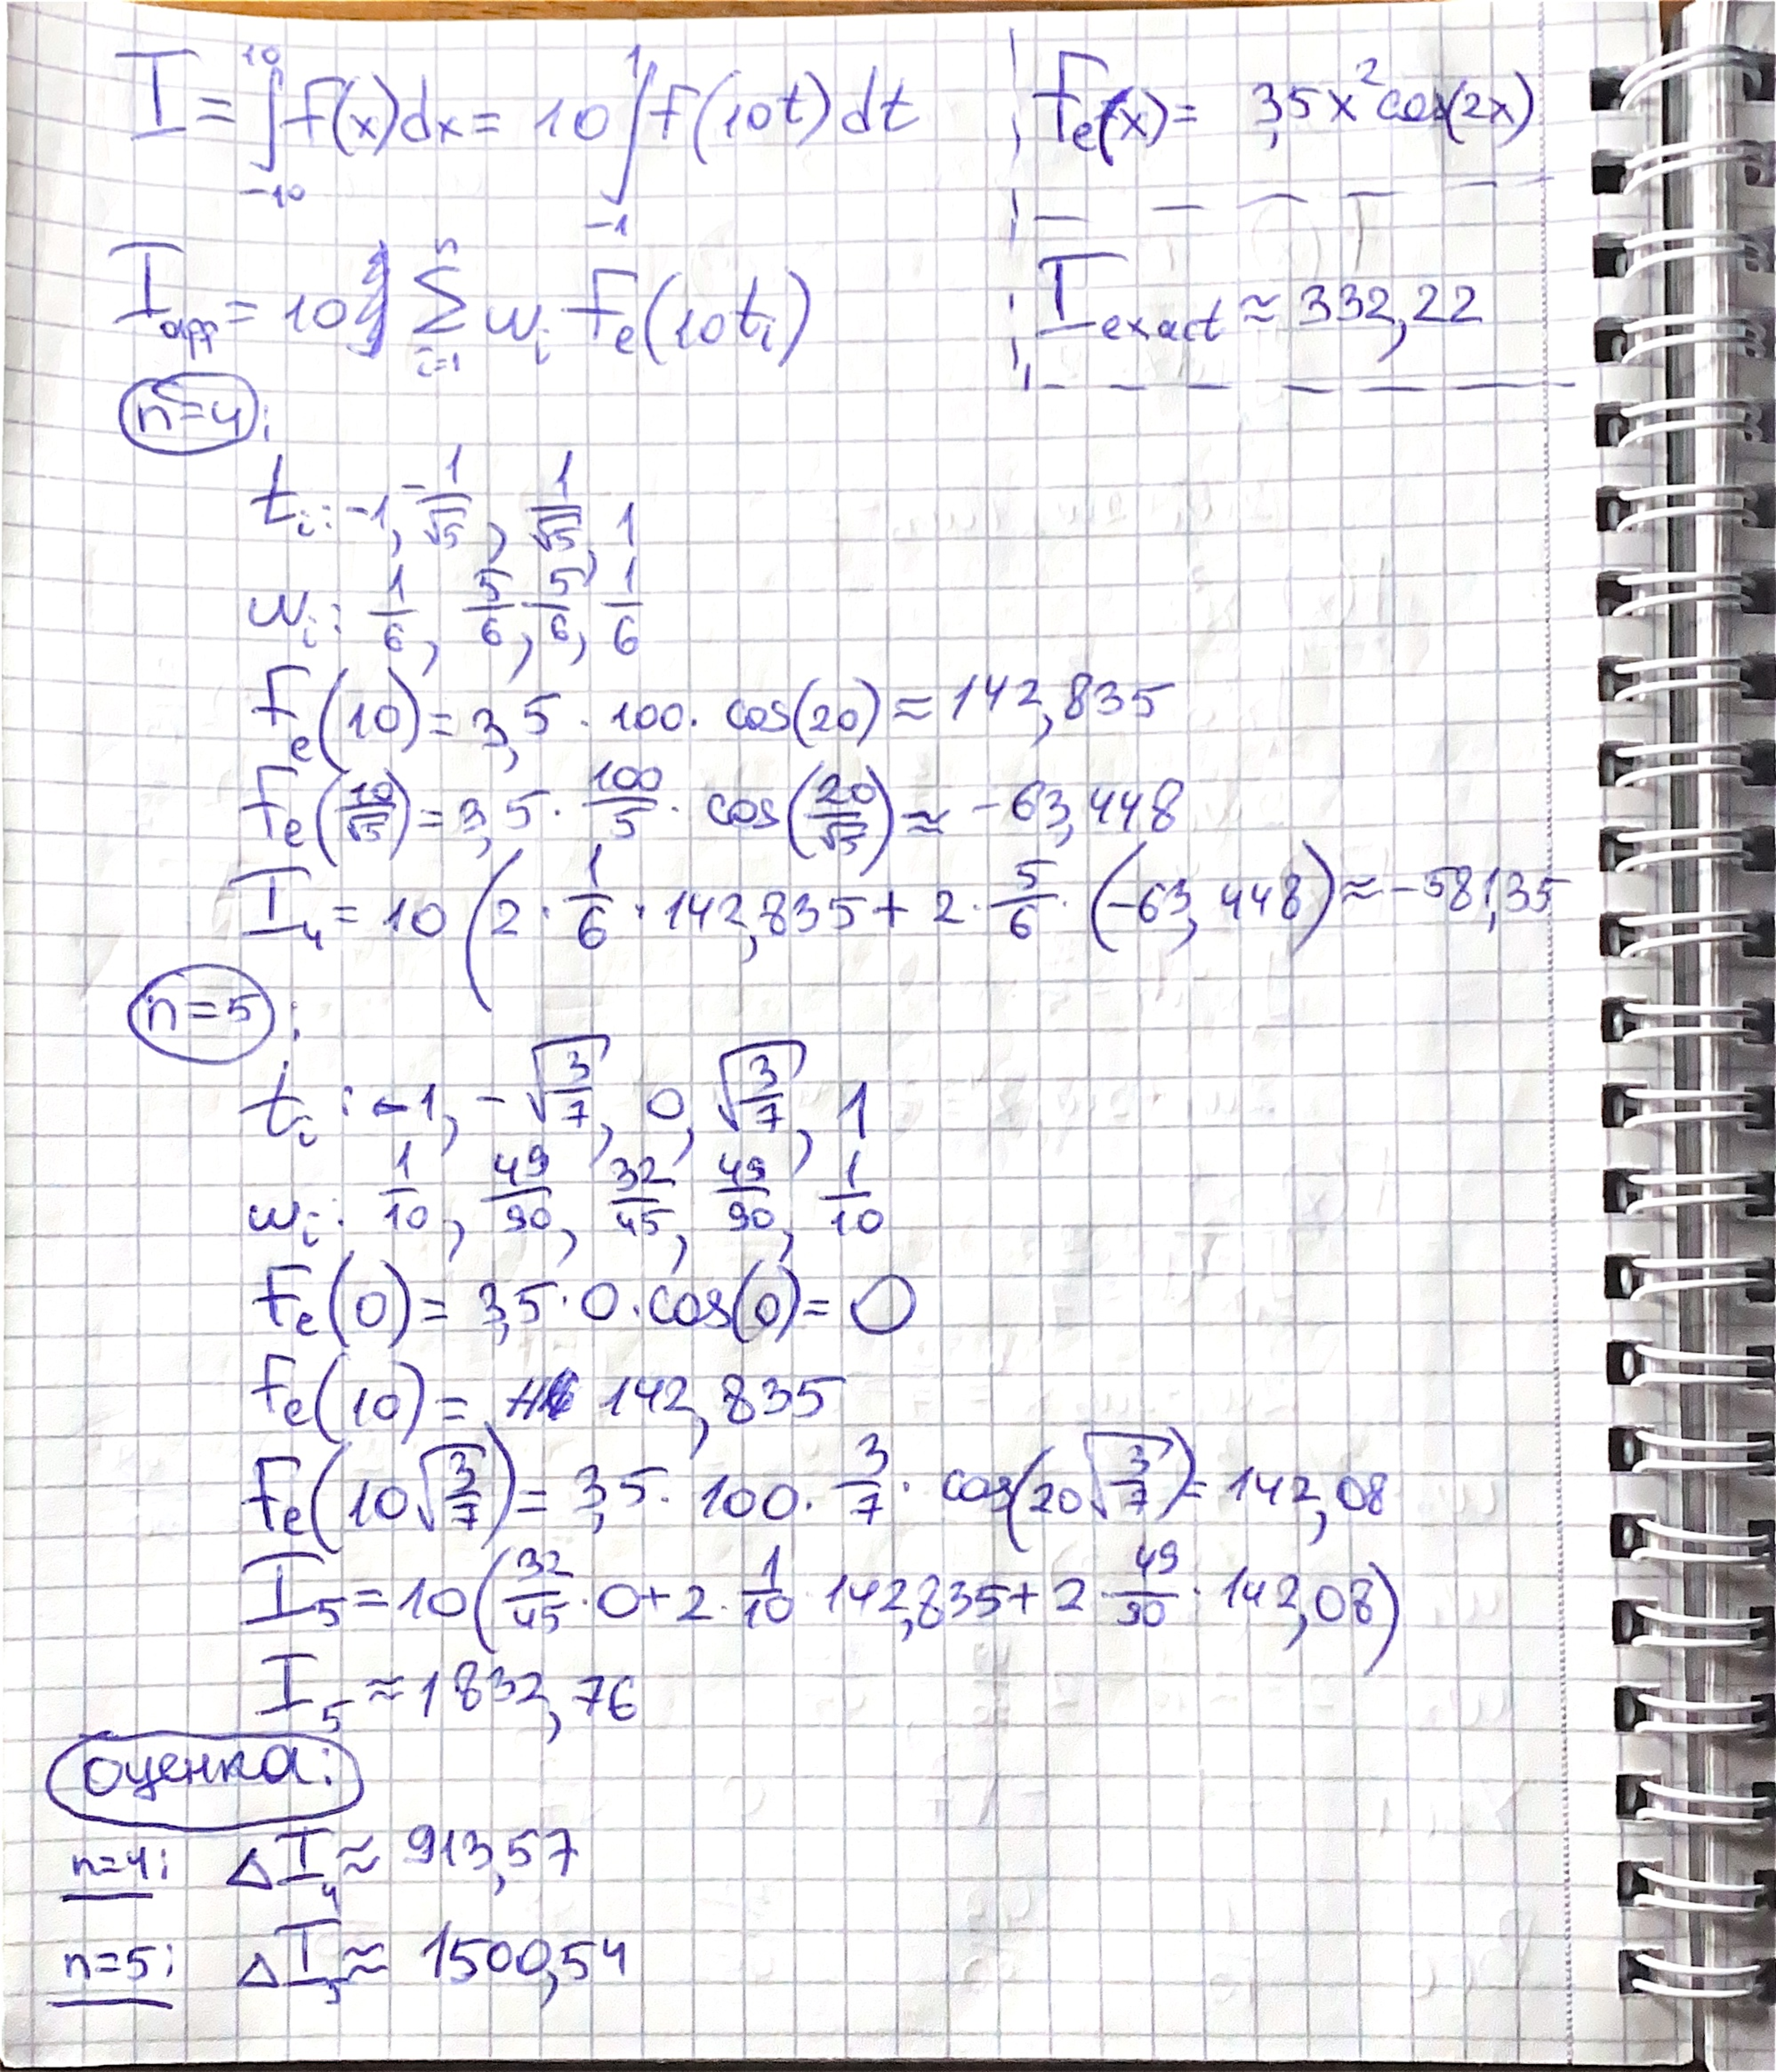
\includegraphics[width=0.92\linewidth]{../data/test_1.pdf}
			\caption{Тестовый пример: Квадратурные формулы Гаусса–Лобатто}
			\label{fig:test_1}
		\end{framed}
	\end{figure}
	
	\begin{figure}[H]
		\centering
		\begin{framed}
			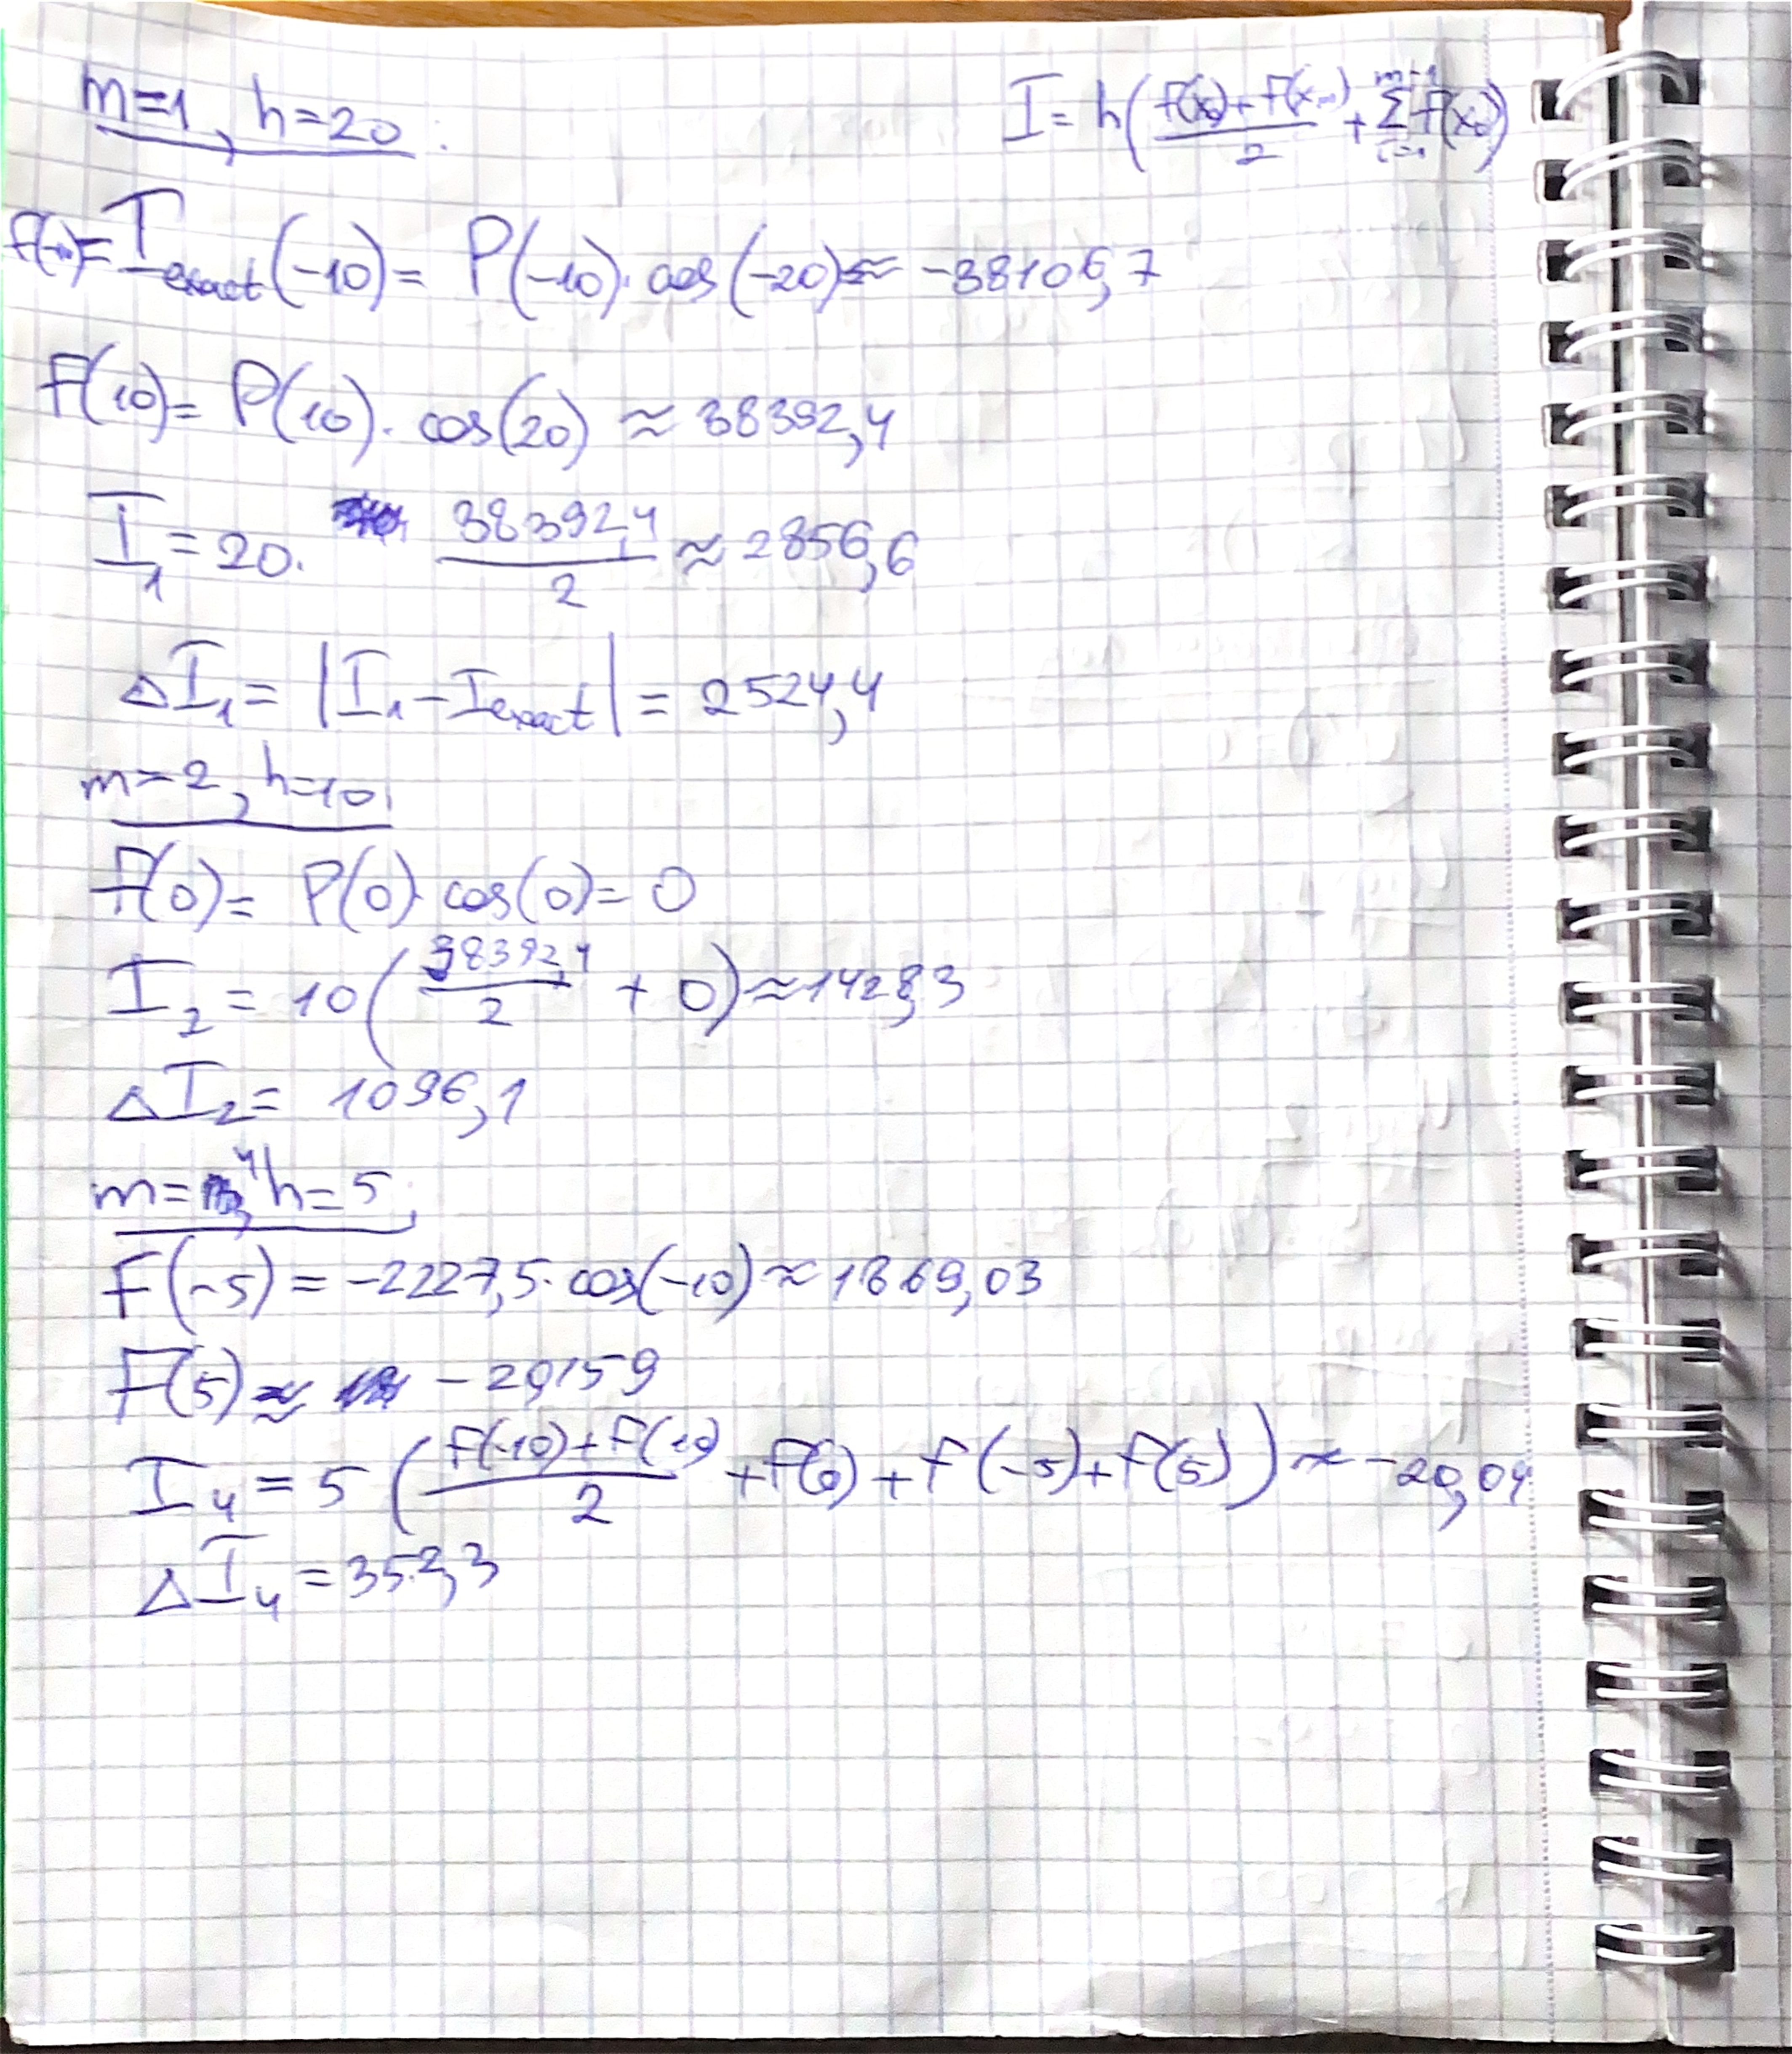
\includegraphics[width=0.92\linewidth]{../data/test_2.pdf}
			\caption{Тестовый пример: Метод трапеций (Ньютон–Котес)}
			\label{fig:test_2}
		\end{framed}
	\end{figure}
	
	На грубых сетках оба метода демонстрируют существенное отклонение от точного значения из-за эффекта ложной дискретизации колебаний $\cos(2x)$
	
	%-------- the fifth point --------
	
	\newpage
	\section{\Large \underline{Подготовка контрольных тестов}}
	
	\begin{itemize}
		\item \textbf{Тестовая функция:}
		\[
		f(x) = (x^5 - 6.2x^3 + 3.5x^2 - 7x)\cos(2x).
		\]
		\item \textbf{Симметрия задачи:}
		Так как $\cos(2x)$ четная, а нечетная часть полинома $P_{\text{odd}}(x) = x^5 - 6.2x^3 - 7x$ интегрируется по симметричному отрезку в ноль, вклад в интеграл дает только четная компонента:
		\[
		I_{\text{exact}} = 7 \int_0^{10} x^2 \cos(2x)\,dx = 348.25 \sin(20) + 35 \cos(20) \approx 332.216055729376.
		\]
		\item \textbf{Критерии контроля:}
		\begin{itemize}
			\item Сравнение численного приближения с точным аналитическим значением;
			\item Мониторинг встроенного счетчика вычислений функции;
			\item Проверка выполнения условия $\Delta \le \varepsilon$.
		\end{itemize}
	\end{itemize}
	
	%-------- the sixth point --------
	
	\section{\Large \underline{Модульная структура программы}}
	
	\begin{itemize}[noitemsep]
		\item \textbf{func(x)} — вычисление подынтегральной функции со встроенным инкрементом статического счетчика вызовов.
		\item \textbf{exact\_integral()} — вычисление точного аналитического интеграла.
		\item \textbf{trapezoidal\_adaptive\_step(...)} — шаг адаптивного метода трапеций с контролем по правилу Рунге.
		\item \textbf{integrate\_trapezoidal\_adaptive(...)} — интерфейсная функция метода трапеций с обнулением счетчика и формированием результата.
		\item \textbf{lobatto\_4 / lobatto\_5} — вычисление квадратур Гаусса–Лобатто на произвольном отрезке.
		\item \textbf{lobatto\_adaptive\_step(...)} — шаг адаптивного бисекционного метода Гаусса–Лобатто.
		\item \textbf{integrate\_lobatto\_adaptive(...)} — интерфейсная функция метода Гаусса–Лобатто.
		\item \textbf{export\_results\_csv(...)} — отдельная функция экспорта результатов серии экспериментов в файл CSV.
	\end{itemize}
	
	%-------- the eighth point --------
	
	\newpage
	\section{\Large \underline{Численный анализ решения задачи}}
	
	В соответствии с заданием по Теме 2 курсовой работы были построены графики и проведен сравнительный анализ двух методов.
	
	\begin{figure}[H]
		\centering
		\begin{framed}
			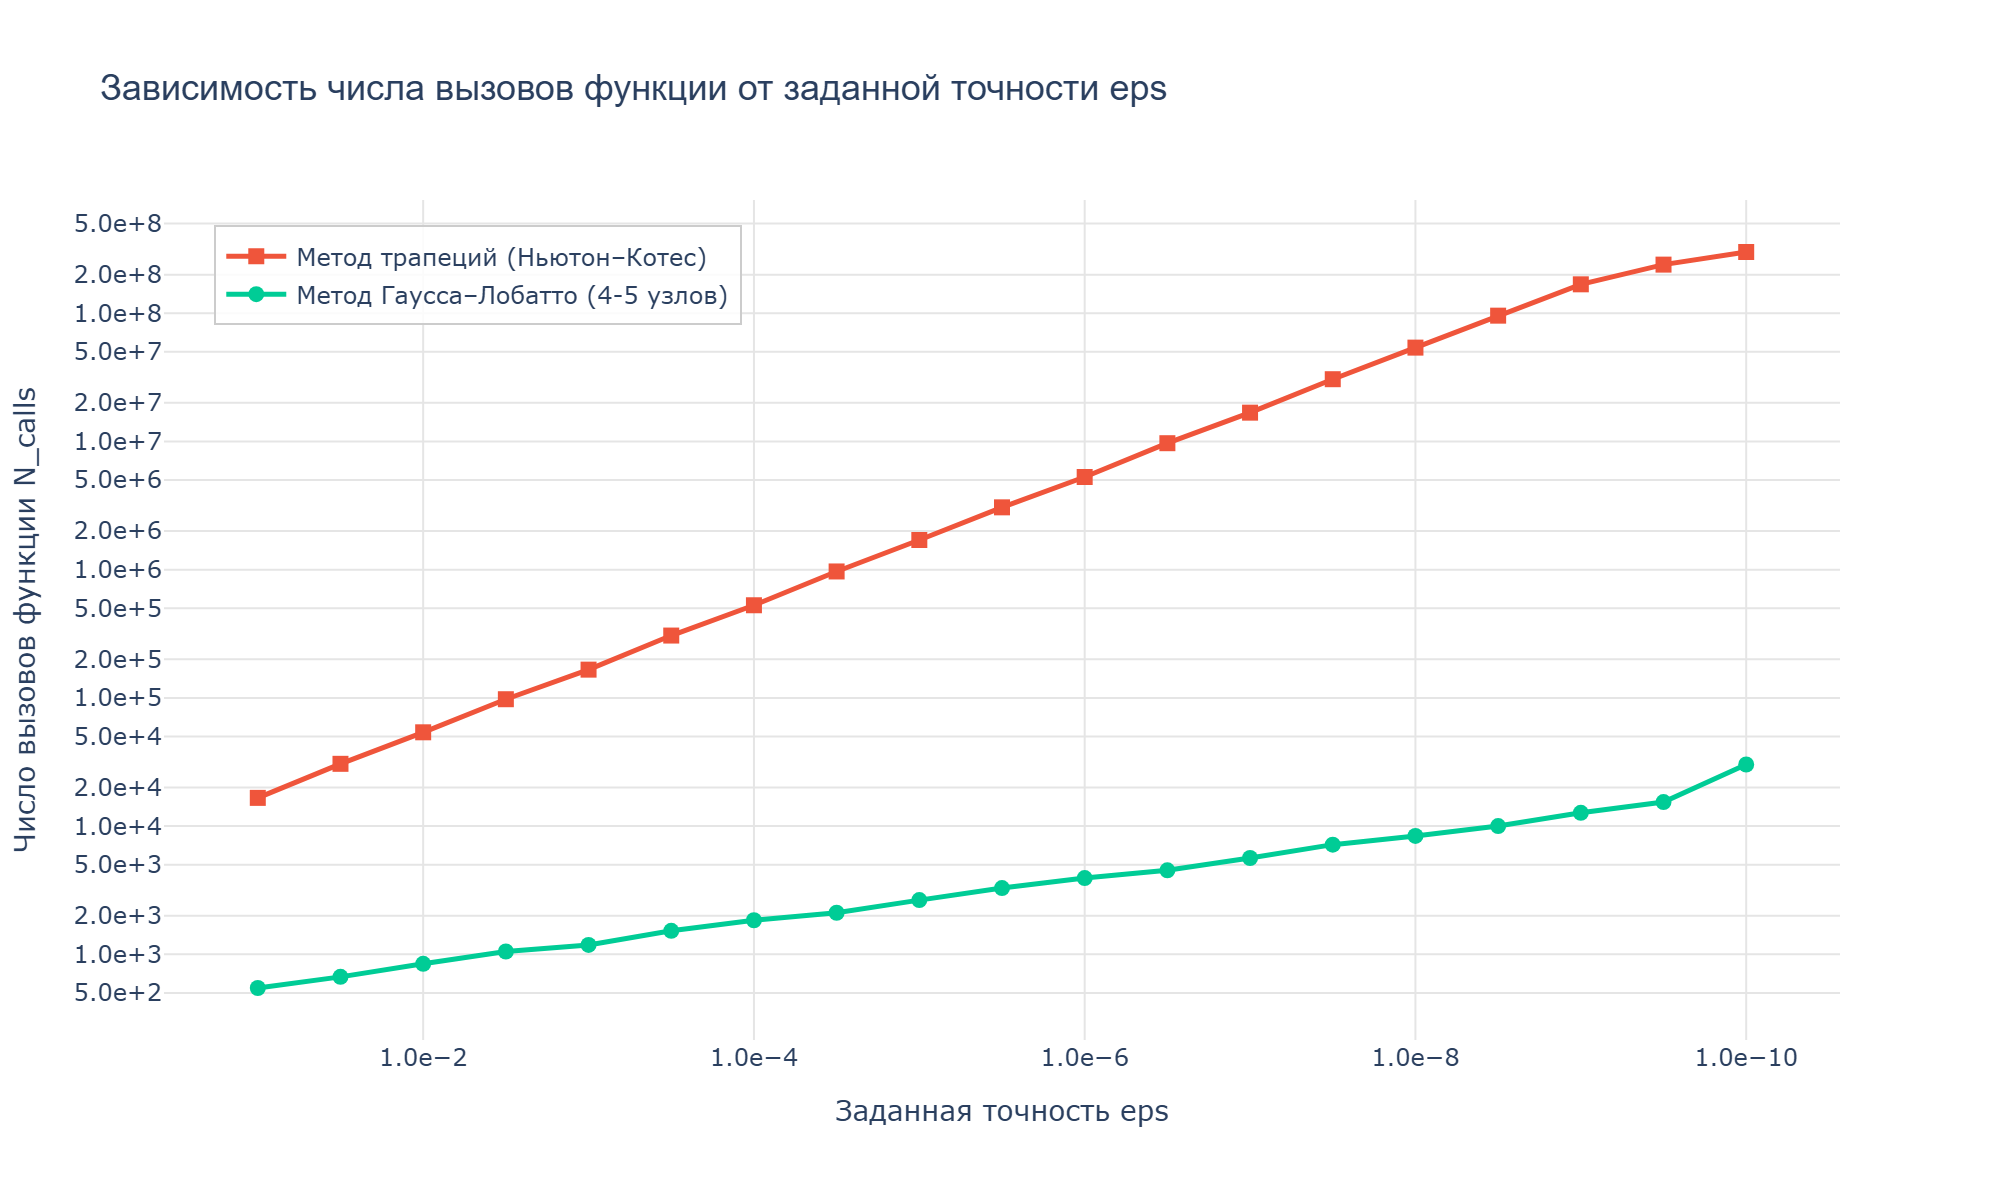
\includegraphics[width=0.92\linewidth]{../data/calls_vs_eps.png}
			\caption{Зависимость количества вызовов функции от заданной точности}
			\label{fig:calls_vs_eps}
		\end{framed}
	\end{figure}
	
	\begin{figure}[H]
		\centering
		\begin{framed}
			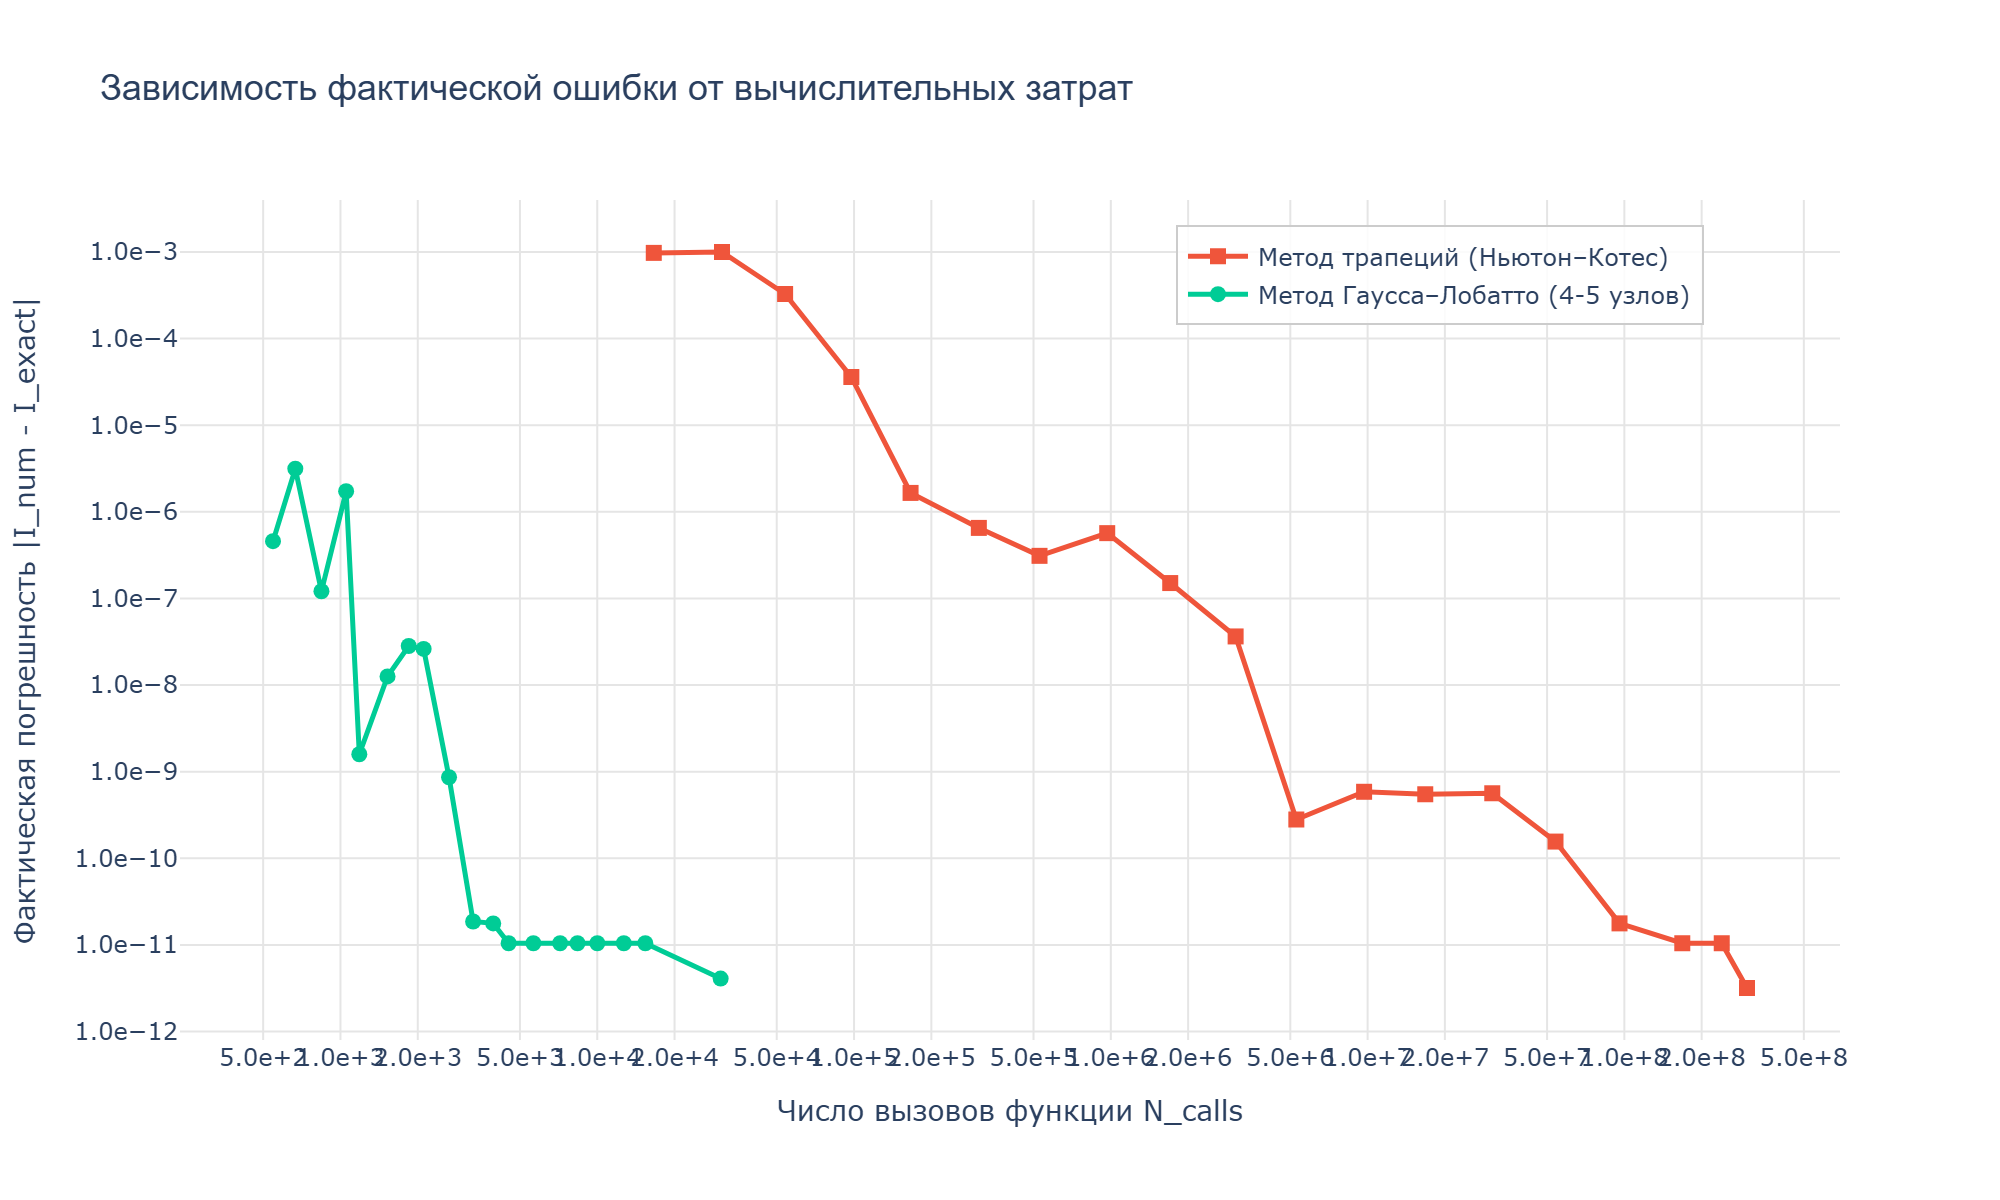
\includegraphics[width=0.92\linewidth]{../data/error_vs_calls.png}
			\caption{Зависимость фактической погрешности от количества вызовов функции}
			\label{fig:error_vs_calls}
		\end{framed}
	\end{figure}
	
	\newpage
	
	\begin{figure}[H]
		\centering
		\begin{framed}
			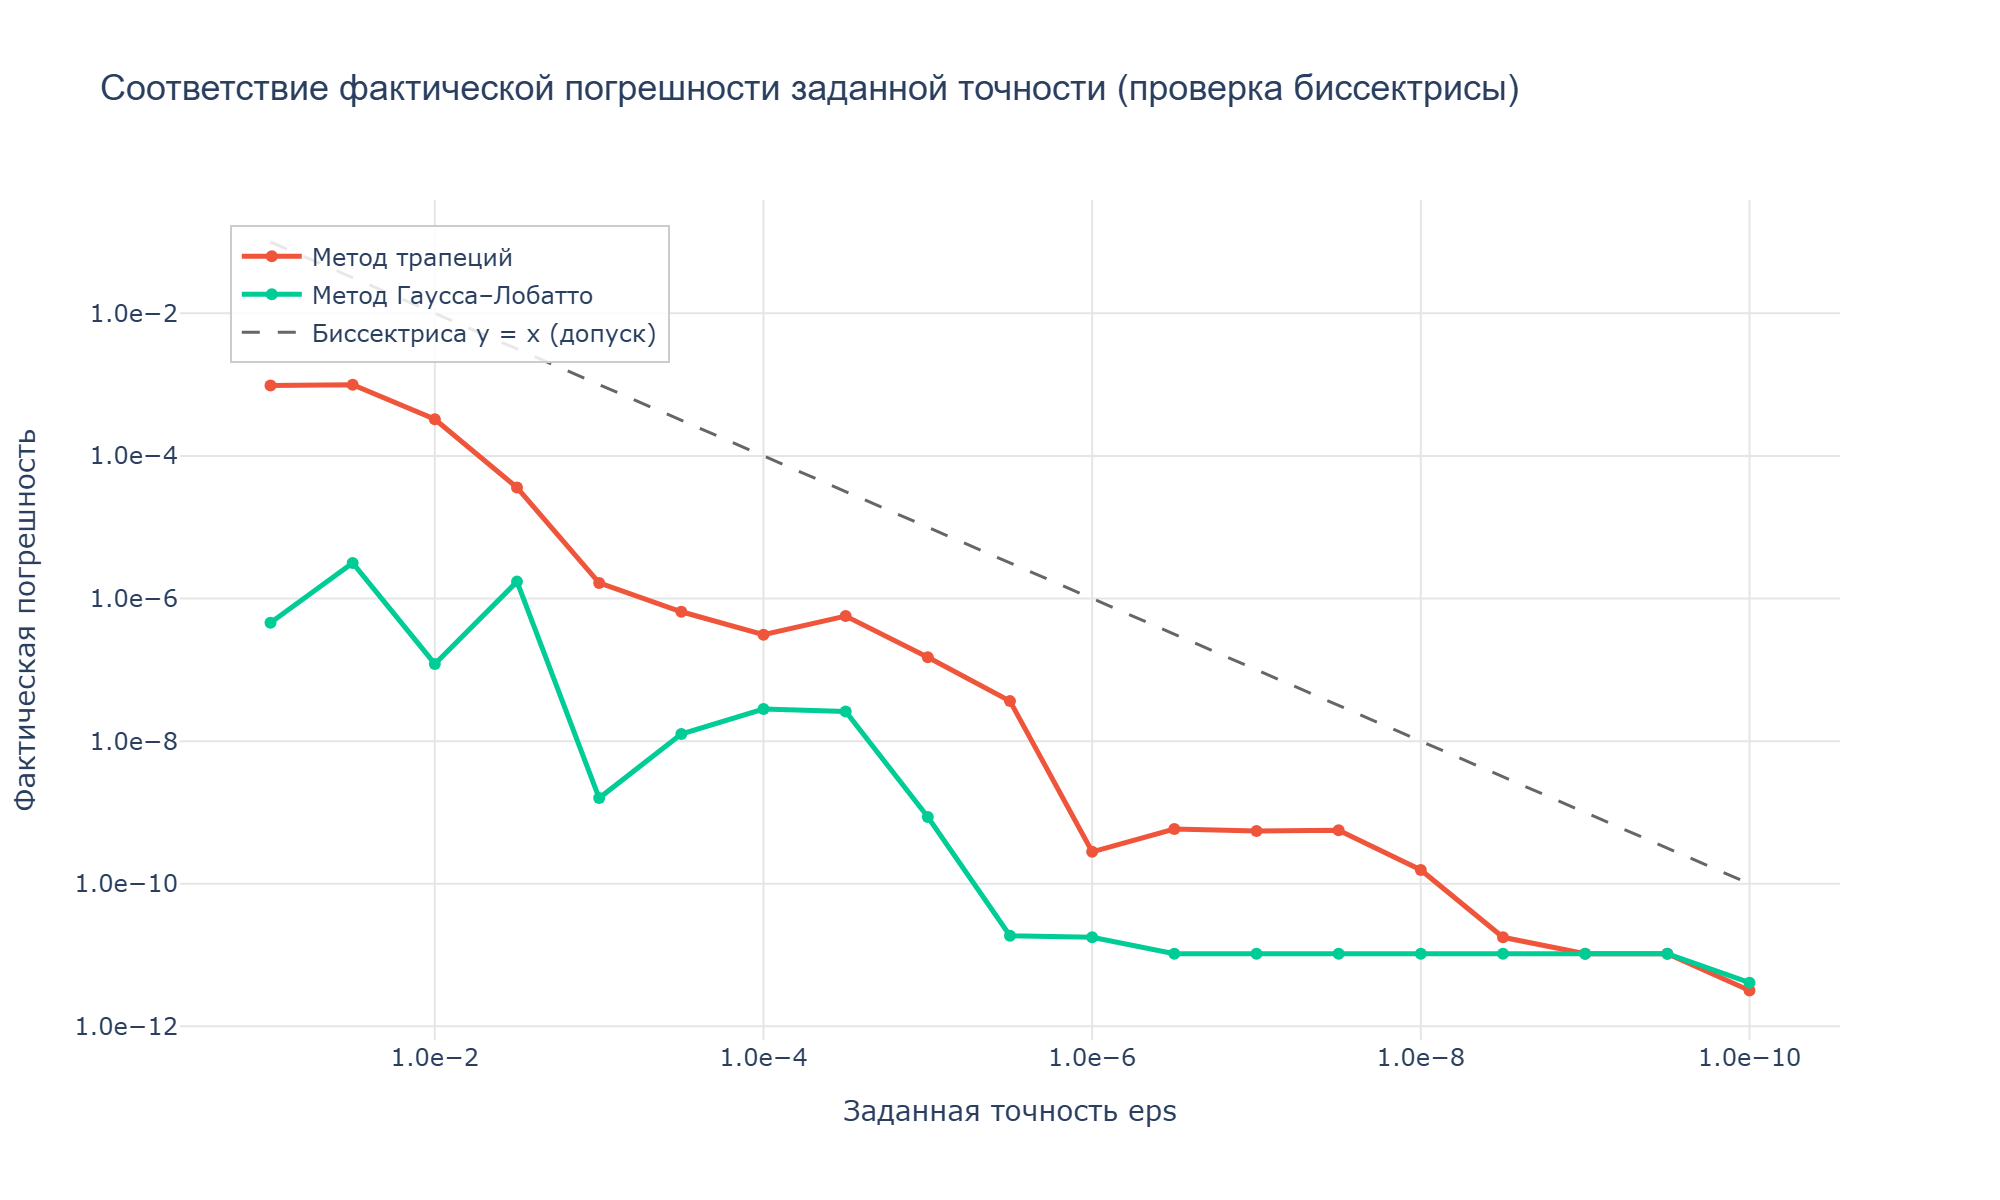
\includegraphics[width=0.92\linewidth]{../data/error_vs_eps.png}
			\caption{Зависимость фактической ошибки от заданной точности}
			\label{fig:error_vs_eps}
		\end{framed}
	\end{figure}
	
	\subsection{Сводная таблица результатов численного эксперимента}
	
	\begin{table}[H]
		\centering
		\caption{Сравнение метода трапеций и метода Гаусса–Лобатто}
		\label{tab:results}
		\small
		\begin{tabular}{|c|c|c|c|c|}
			\hline
			\textbf{Точность} $\varepsilon$ & \textbf{Вызовы (Трапеции)} & \textbf{Ошибка (Трапеции)} & \textbf{Вызовы (Лобатто)} & \textbf{Ошибка (Лобатто)} \\
			\hline
			$1.0 \cdot 10^{-1}$  & $16\,599$        & $9.75 \cdot 10^{-4}$ & $546$    & $4.58 \cdot 10^{-7}$ \\
			$1.0 \cdot 10^{-2}$  & $53\,899$        & $3.27 \cdot 10^{-4}$ & $843$    & $1.21 \cdot 10^{-7}$ \\
			$1.0 \cdot 10^{-4}$  & $527\,655$       & $3.10 \cdot 10^{-7}$ & $1\,844$ & $2.82 \cdot 10^{-8}$ \\
			$1.0 \cdot 10^{-6}$  & $5\,278\,389$    & $2.81 \cdot 10^{-10}$ & $3\,934$ & $1.77 \cdot 10^{-11}$ \\
			$1.0 \cdot 10^{-8}$  & $53\,925\,723$   & $1.56 \cdot 10^{-10}$ & $8\,378$ & $1.05 \cdot 10^{-11}$ \\
			$1.0 \cdot 10^{-10}$ & $300\,319\,045$  & $3.18 \cdot 10^{-12}$ & $30\,235$ & $4.09 \cdot 10^{-12}$ \\
			\hline
		\end{tabular}
	\end{table}
	
	\subsection{Анализ результатов}
	
	\begin{enumerate}
		\item \textbf{Зависимость числа вызовов от точности (рис.~\ref{fig:calls_vs_eps}):}
		Для достижения точности $\varepsilon = 10^{-10}$ методу трапеций потребовалось более $3 \cdot 10^8$ вызовов функции, тогда как адаптивному методу Гаусса–Лобатто — всего $30\,235$ вызовов. Выигрыш метода Лобатто по вычислительным ресурсам составляет четыре порядка ($\approx 10\,000$ раз).
		
		\item \textbf{Зависимость ошибки от числа вызовов (рис.~\ref{fig:error_vs_calls}):}
		В логарифмических координатах метод Гаусса–Лобатто демонстрирует несравненно более крутой наклон прямой ошибки, что отражает его высокий алгебраический порядок точности ($p = 7$ против $p = 2$ у метода трапеций).
		
		\item \textbf{Проверка критерия останова (рис.~\ref{fig:error_vs_eps}):}
		Линии фактической погрешности обоих методов располагаются строго ниже биссектрисы $y = x$, что доказывает надёжность используемых адаптивных критериев останова.
	\end{enumerate}
	
	%-------- the ninth point --------
	
	\newpage
	\section{\Large \underline{Выводы}}
	
	В ходе выполнения курсовой работы по Теме 2 был проведён сравнительный численный анализ эффективности метода трапеций (Ньютон–Котес) и метода Гаусса–Лобатто:
	
	\begin{itemize}
		\item Доказано кардинальное преимущество квадратур типа Гаусса–Лобатто: за счёт оптимального расположения внутренних узлов метод обеспечивает экспоненциально более высокую скорость сходимости, сокращая число вычислений функции в тысячи раз по сравнению с методом трапеций.
		\item Полученные численные результаты полностью согласуются с теоретическими оценками порядков аппроксимации.
	\end{itemize}
	
\end{document}
